\documentclass[border=4pt]{standalone}
% Preámbulo común de las figuras. Cada figura es un documento standalone
% que se compila a SVG con scripts/build_figures.sh
\usepackage[utf8]{inputenc}
\usepackage{amsmath}
\usepackage{tikz}
\usepackage[american, siunitx]{circuitikz}
\usetikzlibrary{arrows.meta,calc,decorations.pathmorphing,patterns}
\tikzset{
  >={Stealth[length=2.2mm]},
  eje/.style={->, thin},
  hilo/.style={thick},
}
% Paleta común: tonos medios legibles sobre fondo claro
\definecolor{azul}{RGB}{31,94,168}
\definecolor{rojo}{RGB}{192,57,43}
\definecolor{verde}{RGB}{39,128,73}
\definecolor{naranja}{RGB}{211,120,30}
\definecolor{morado}{RGB}{125,60,152}

\begin{document}
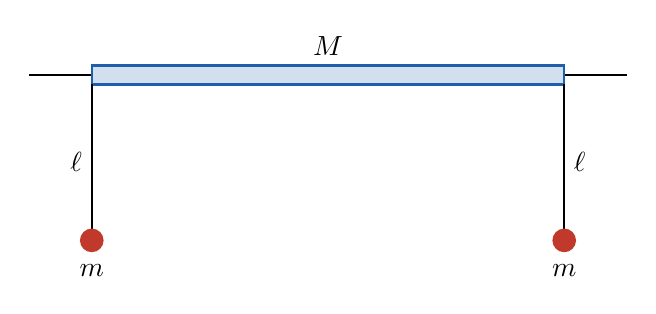
\begin{tikzpicture}[scale=1.0]
  \draw[thick] (-0.8,2.5) -- (6.8,2.5);
  \filldraw[draw=azul, fill=azul!20, thick] (0,2.38) rectangle (6,2.62);
  \node[above] at (3,2.62) {$M$};
  \draw[hilo] (0,2.38) -- (0,0.4);
  \draw[hilo] (6,2.38) -- (6,0.4);
  \fill[rojo] (0,0.4) circle (0.15);
  \fill[rojo] (6,0.4) circle (0.15);
  \node[below] at (0,0.22) {$m$};
  \node[below] at (6,0.22) {$m$};
  \node[left] at (0,1.4) {$\ell$};
  \node[right] at (6,1.4) {$\ell$};
\end{tikzpicture}
\end{document}
